% https://tex.stackexchange.com/questions/287672/
\backgroundsetup{%
  scale=1,
  angle=0,
  contents={%
    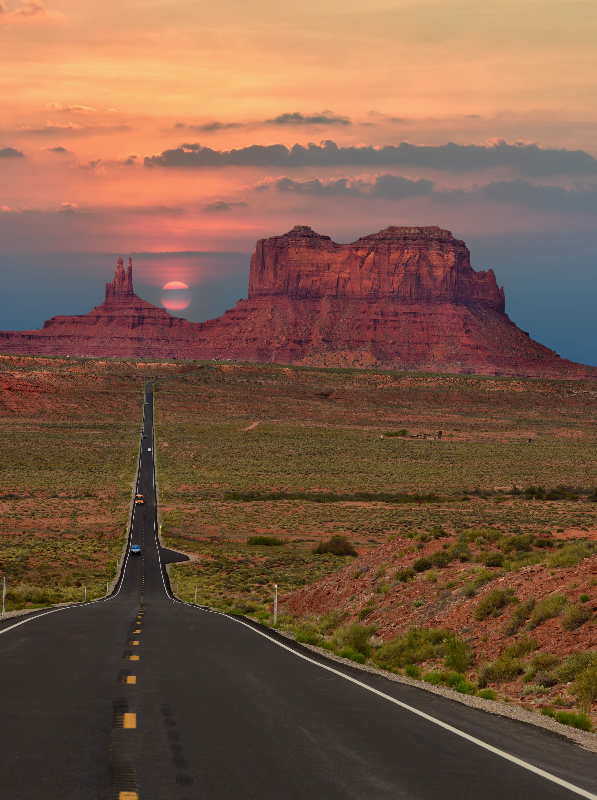
\includegraphics[width=\paperwidth,
                     height=\paperheight]{luaking_title4.png}
  },
  position=current page.north east,
  opacity=1,
  anchor=below left,
  }

\begin{titlepage}
\BgThispage
  \begin{center}
    \vspace*{2cm}
    % {\fontsize{32}{40}\selectfont\textcolor{white}{\textbf{LUAKING}}\par}
    
\includegraphics[width=0.9\linewidth]{luaking_title2.png}\par
    \vspace{1cm}
    
\includegraphics[width=0.8\linewidth]{luaking_title3.png}\par
    \vspace{1cm}
    {\textcolor{black!5}{\Large\textsc{Jaroslav Fait}}\par}
    \vspace{1\baselineskip}
    {\textcolor{black!5}{\large\today}\par}
    \vfill
    {\textcolor{black!10}{University of West Bohemia}\par}
    {\textcolor{black!10}{Faculty of Electrical Engineering}\par}
    \vspace{0.3cm}
    {\textcolor{black!10}{\footnotesize\luatexbanner}\par}
    {\textcolor{black!10}{\footnotesize and also \KOMAScriptVersion}}
    \vspace*{0.3cm} 
    % \hrule
  \end{center}
\end{titlepage}